\documentclass[border=3pt]{standalone}

% Drawing
\usepackage{tikz}

% Tikz Library
\usetikzlibrary{3d, shapes.multipart}

% Styles
\tikzset{>=latex} % for LaTeX arrow head
\tikzset{axis/.style={black, thick,->}}
\tikzset{vector/.style={>=stealth,->}}
\tikzset{every text node part/.style={align=center}}

% New Command
%% Viewing Screen
\newcommand{\rect}[1]{%
	\begin{scope}[canvas is xz plane at y=1.2]
		\draw[thick, fill=black!40] (#1,-1.2) rectangle (#1+0.2,1.2);
	\end{scope}
	%
	\begin{scope}[canvas is xy plane at z=1.2]
		\draw[thick, fill=black!25](#1,-1.2) rectangle (#1+0.2,1.2);
	\end{scope}
	%
	\begin{scope}[canvas is yz plane at x=#1]
		\draw[thick, fill=black!10] (-1.2,-1.2) rectangle (1.2,1.2);
		\draw[thick, fill=black!10, dashed] (0,0) circle (0.65cm);
		\foreach \i in {0,45,...,360}
		{
			\draw[thick, dashed] (0,0) -- ({0.65*cos(\i)}, {0.65*sin(\i)});
		}
	\end{scope}
}
%% Draw Line in Polar Coordinates from (0,0) to (t,theta)
\newcommand{\cdraw}[2]{\draw[very thick, -stealth, red] (0,0) -- ({#1*cos(#2)}, {#1*sin(#2)});}

% Notation
\usepackage{amsmath}

\begin{document}

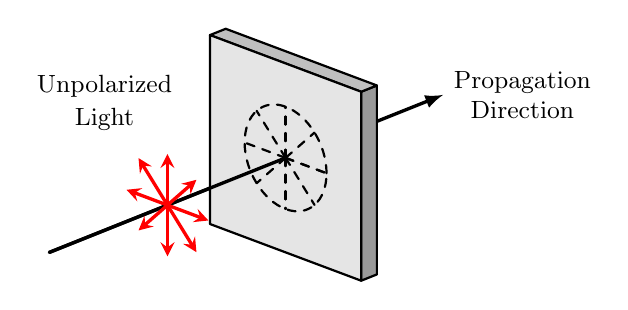
\begin{tikzpicture}[x={(1cm,0.4cm)}, y={(8mm, -3mm)}, z={(0cm,1cm)}, line cap=round, line join=round]
	
	% Main Axes
%	\draw[->] (0,0,0) -- (6,0,0) node[right] {$x$};
%	\draw[->] (0,0,0) -- (0,2,0) node[below left] {$y$};
%	\draw[->] (0,0,0) -- (0,0,2) node[above] {$z$};

	% Propagation Direction
	\draw[very thick, ->] (1,0,0) -- (6,0,0) node[right, black] {\small{Propagation}\\[-0.5mm]\small{Direction}};
	
	% Viewing Screen
	\rect{4}
	
	% Refinements to Look 3D	
	\draw[very thick] (1,0,0) -- (4,0,0);
	
	\begin{scope}[canvas is yz plane at x=2.5]		
		\cdraw{0.65}{0}
		\cdraw{0.65}{45}
		\cdraw{0.65}{90}
		\cdraw{0.65}{135}
		\cdraw{0.65}{180}
		\cdraw{0.65}{225}
		\cdraw{0.65}{270}
		\cdraw{0.65}{315}
	\end{scope}
	
	% Nodes
	\node at (2.5,-1,1) {\small{Unpolarized}\\\small{Light}};
\end{tikzpicture}

\end{document}
